\documentclass{article}
\usepackage{spconf,amsmath,graphicx}
\usepackage{url}
\usepackage{hyperref}
\def\x{{\mathbf x}}
\def\L{{\cal L}}
\title{GTA Course Project Report : Viewing Implicit Social Network as Bipartite Graphs}
%
% Single address.
% ---------------
\name{Mohan Kumar (MT19AIE265)}
\address{IIT Jodhpur}
\begin{document}
%\ninept
%
\maketitle
%
\begin{abstract}
The indirect social networks developed in today's worlds are generally defined latent when users on any social network or any socially active website interact by giving their inputs on a common or shared object. This model consists of a bipartite graph where users and interaction points are two different classes of nodes, which are connected by edges when the users interact with a shared object. Therefore such a modelled bipartite graph contains significant useful information on the indirect social network and can be effectively used for analysing and visualising these network data structures. This is how social websites and applications recommends the friends or connections. Some social websites and applications like linkedin also predict about the jobs one may be interested. They are generally very useful in studying the Social Networks where people act as nodes of the network and determine how connected the two profiles are by various parameters helping them in recommending the jobs and further proceed for social connections.
\end{abstract}

\begin{keywords}
social networks, social bipartite graphs, graph theory with intelligence.
\end{keywords}

\section{Introduction}
Social network analysis can help prevent spreading of rumours and abuse on social sites and other socially active applications by detecting the important nodes in different social platforms which when actively taken care of will minimize the spread of a particular rumour and various non-appropriate behaviours. In this project we will study about the various Node and Edge attributes of a social network with different types of graphs and different parameters that generally describe the social networks in to-days context. For the given problem statement we will provide a case study using some references of papers and will try to demonstrate in python with the following attributes:
\begin{itemize}
  \item Concepts of bipartite graphs.
  \item Using the node and edge parameters of graphs
  \item Clustering and distance measures
\end{itemize}
A bipartite graph can represent users and interaction points as two different classes of nodes, which are connected by edges when the users interact with the common shared object.
Node and edge parameters of graphs can be weighted to determine the strength of relation between nodes and edges as shown in fig.1.
\begin{figure}[ht]
\centering
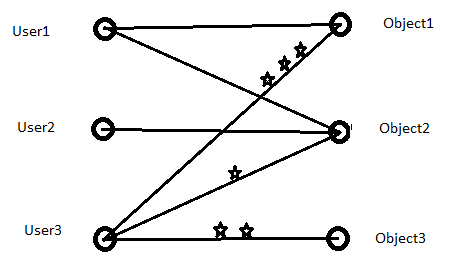
\includegraphics[scale=0.6]{bipar2.png}
\caption{Bipartite Graph Model}
\end{figure}
Clustering parameter describes the pair of Node’s friend that are friends with each other representing the degree to which the nodes in the whole network tend to cluster.

\newpage
\newpage

\section{Related Works}
Bipartite Graphs generally have two sets one for users and other for the services or objects that the users have connected in the past. To create the graph between users which share the common objects and would be using a weighted graph where weights are proportional to the objects they have in common, thus making it a projected graph and so if someone connects to a new object then one can recommend that object to the users which share an edge in such a projected graph with that user.
\newline
We used 'networkx' package in python environment to demonstrate and analyse this model.
To find out the distance of a nodes from a given node BFS algorithm is used. In Networkx python library we can use nx.bfs.tree('N2',’N1’) statement to get distances from node N1.
\newline
Therefore, to compare the closeness of different nodes in a network and compare groups based on degree of closeness between their members can be computed by Average distance between a pair of nodes by the python library named network, nx.average.shortest.path.length(G).
\newline
The main concern in such social network is to avoid spreading of rumours on network which can be achieved by centrality distance measures of the important nodes in the network.
\newline
For modeling this we need to generate the Graph between users which share the common connection-object and this would be a weighted graph where weights would be proportional to how many objects they commonly share and this graph is now termed as Projected Graph. Therefore, when a user connects to some new object we can recommend that object to the other users which share an edge in the Projected Graph with that user.

\newpage

\section{Definitions}
Edges connecting different nodes can be weighed to determine the strength of connections between nodes and they can thus be given different relations like family, friend etc.
\newline
Graphs with edges that do not have a direction are termed as Undirected Graphs. The edges indicate a two-way connection between the nodes, in that each edge can be traversed in both directions. 
\newline
Whereas, the graphs having edges with direction are termed as Directed Graphs. The edges indicate a one-way connection only and each edge in this case can be traversed in one direction only.
\newline
The number of nodes that the given node is connected to is termed as its degree. There are two types of degree ‘In-degree’ and ‘Out-degree’ which comes into picture in directed graph.
\newline
The Graphs whose nodes can be split into two groups \({G_1}\) and \({G_2}\) and each edge is connected to the node from \({G_1}\) to a node of \({G_2}\), are termed as Bipartite Graphs.
Considering there are seven users and four Teams and as this graph is split into two groups of nodes, it becomes a Bipartite Graph as shown in the fig.2.
\begin{figure}[ht]
\centering
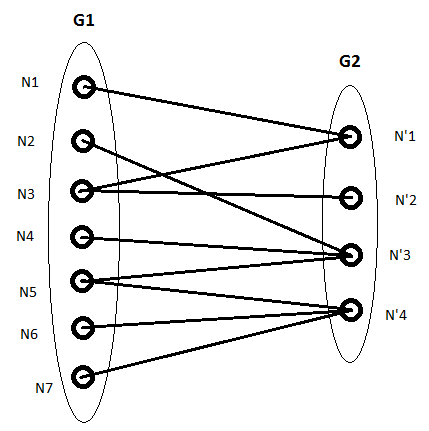
\includegraphics[scale=0.6]{bipar1.png}
\caption{Bipartite Graph}
\end{figure}
\newpage

\section{Case Study using python}
For this analysis we are using a Python package NetworkX which is widely used for the creation, manipulation, and study of the structure, dynamics, and functions of complex networks. For the features creation and predicting the links between different users we are using 'sklearn' package.
\newline
If we consider a Social Network where people are connected to each other, we can get some information about the network based on existing connections between the peoples and then we can predict further connections that can thus be generated in the network.
\newline
We have taken a Facebook data-set from Stanford University site which is having the aggregated network of ten individuals’ Facebook friends list. We will read the file and construct the graphs for this analysis. This data-set network consists of 4,039 nodes, connected with 88,234 edges.
\newline
We have taken different link prediction measures like betweenness, degree, closeness centrality, finding the shortest path for the nodes etc. 
\begin{figure}[ht]
\centering
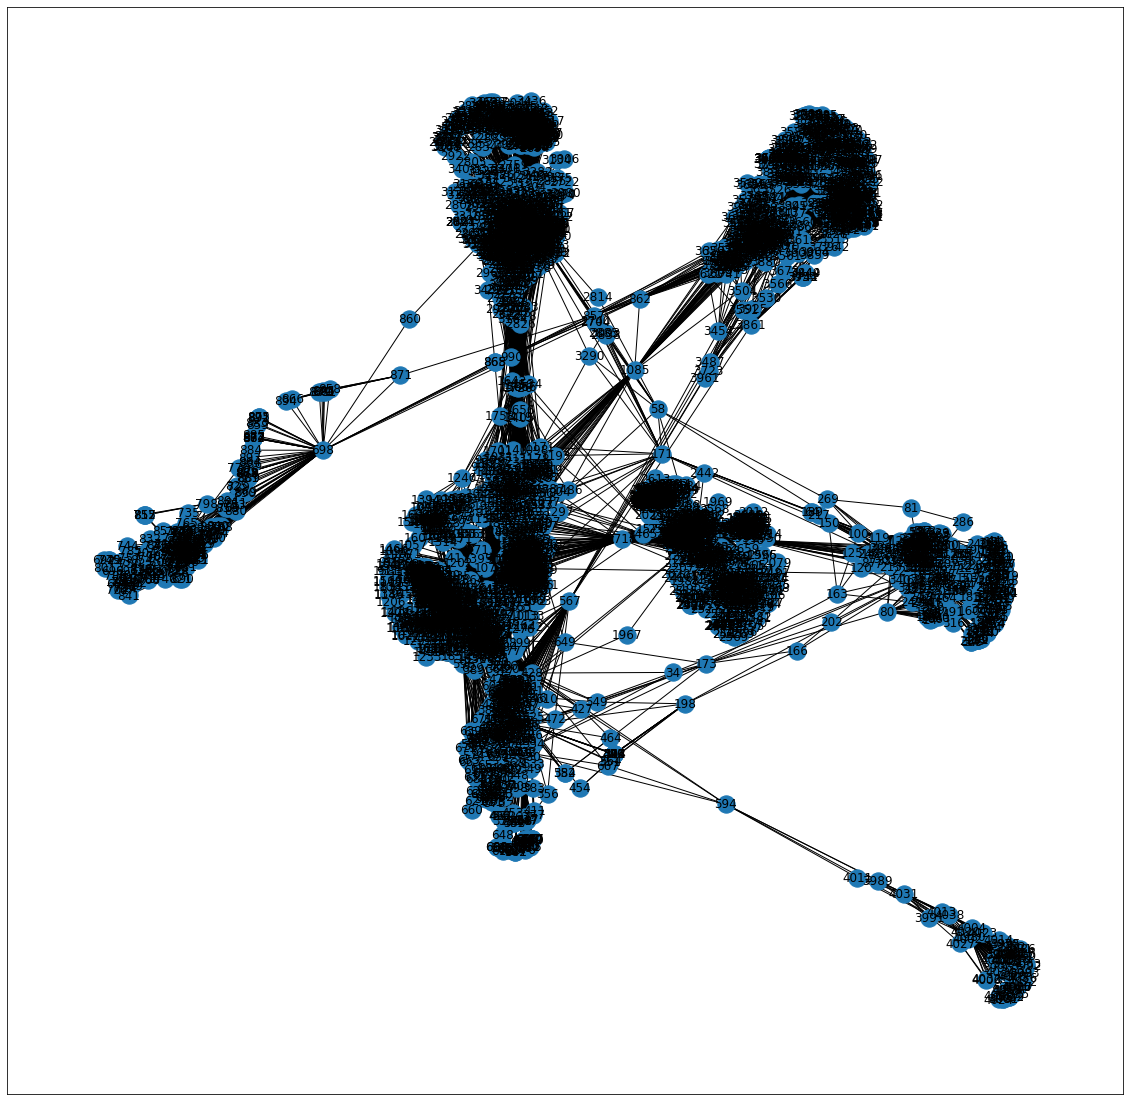
\includegraphics[scale=0.22]{sos_net.png}
\caption{Social Network data points connections}
\end{figure}

\section{Summary}
This analysis rendered us the way to think in terms of todays need in social networks that the graph nodes are things which we are interested in and edges denote the relationships between the things that we are interested in. Thus investigating a graph's edges is the more interesting part of network or graph analysis.
\newline
The key takeaways from this analysis are the Modeling of a problem as a network and to extract useful information from the network.

\bibliographystyle{IEEEbib}
\bibliography{strings,refs}
https://api.semanticscholar.org/CorpusID:13614375
\newline
https://snap.stanford.edu/data/index.html
\newline
https://snap.stanford.edu/data/ego-Facebook.html
\newline
https://networkx.org/
\end{document}
